\documentclass[ignorenonframetext,]{beamer}
\setbeamertemplate{caption}[numbered]
\setbeamertemplate{caption label separator}{: }
\setbeamercolor{caption name}{fg=normal text.fg}
\beamertemplatenavigationsymbolsempty
\usepackage{lmodern}
\usepackage{amssymb,amsmath}
\usepackage{ifxetex,ifluatex}
\usepackage{fixltx2e} % provides \textsubscript
\ifnum 0\ifxetex 1\fi\ifluatex 1\fi=0 % if pdftex
  \usepackage[T1]{fontenc}
  \usepackage[utf8]{inputenc}
\else % if luatex or xelatex
  \ifxetex
    \usepackage{mathspec}
  \else
    \usepackage{fontspec}
  \fi
  \defaultfontfeatures{Ligatures=TeX,Scale=MatchLowercase}
\fi
\usetheme[]{boxes}
\usecolortheme{structure}
% use upquote if available, for straight quotes in verbatim environments
\IfFileExists{upquote.sty}{\usepackage{upquote}}{}
% use microtype if available
\IfFileExists{microtype.sty}{%
\usepackage{microtype}
\UseMicrotypeSet[protrusion]{basicmath} % disable protrusion for tt fonts
}{}
\newif\ifbibliography
\hypersetup{
            pdftitle={miniBeamer package presentation},
            pdfauthor={Bartek Granat \textbar{} Mateusz Polakowski \textbar{} Adam Rydelek \textbar{} Michał Stawikowski \textbar{} Witold Merkel},
            pdfborder={0 0 0},
            breaklinks=true}
\urlstyle{same}  % don't use monospace font for urls
\usepackage{color}
\usepackage{fancyvrb}
\newcommand{\VerbBar}{|}
\newcommand{\VERB}{\Verb[commandchars=\\\{\}]}
\DefineVerbatimEnvironment{Highlighting}{Verbatim}{commandchars=\\\{\}}
% Add ',fontsize=\small' for more characters per line
\newenvironment{Shaded}{}{}
\newcommand{\KeywordTok}[1]{\textcolor[rgb]{0.00,0.00,1.00}{#1}}
\newcommand{\DataTypeTok}[1]{#1}
\newcommand{\DecValTok}[1]{#1}
\newcommand{\BaseNTok}[1]{#1}
\newcommand{\FloatTok}[1]{#1}
\newcommand{\ConstantTok}[1]{#1}
\newcommand{\CharTok}[1]{\textcolor[rgb]{0.00,0.50,0.50}{#1}}
\newcommand{\SpecialCharTok}[1]{\textcolor[rgb]{0.00,0.50,0.50}{#1}}
\newcommand{\StringTok}[1]{\textcolor[rgb]{0.00,0.50,0.50}{#1}}
\newcommand{\VerbatimStringTok}[1]{\textcolor[rgb]{0.00,0.50,0.50}{#1}}
\newcommand{\SpecialStringTok}[1]{\textcolor[rgb]{0.00,0.50,0.50}{#1}}
\newcommand{\ImportTok}[1]{#1}
\newcommand{\CommentTok}[1]{\textcolor[rgb]{0.00,0.50,0.00}{#1}}
\newcommand{\DocumentationTok}[1]{\textcolor[rgb]{0.00,0.50,0.00}{#1}}
\newcommand{\AnnotationTok}[1]{\textcolor[rgb]{0.00,0.50,0.00}{#1}}
\newcommand{\CommentVarTok}[1]{\textcolor[rgb]{0.00,0.50,0.00}{#1}}
\newcommand{\OtherTok}[1]{\textcolor[rgb]{1.00,0.25,0.00}{#1}}
\newcommand{\FunctionTok}[1]{#1}
\newcommand{\VariableTok}[1]{#1}
\newcommand{\ControlFlowTok}[1]{\textcolor[rgb]{0.00,0.00,1.00}{#1}}
\newcommand{\OperatorTok}[1]{#1}
\newcommand{\BuiltInTok}[1]{#1}
\newcommand{\ExtensionTok}[1]{#1}
\newcommand{\PreprocessorTok}[1]{\textcolor[rgb]{1.00,0.25,0.00}{#1}}
\newcommand{\AttributeTok}[1]{#1}
\newcommand{\RegionMarkerTok}[1]{#1}
\newcommand{\InformationTok}[1]{\textcolor[rgb]{0.00,0.50,0.00}{#1}}
\newcommand{\WarningTok}[1]{\textcolor[rgb]{0.00,0.50,0.00}{\textbf{#1}}}
\newcommand{\AlertTok}[1]{\textcolor[rgb]{1.00,0.00,0.00}{#1}}
\newcommand{\ErrorTok}[1]{\textcolor[rgb]{1.00,0.00,0.00}{\textbf{#1}}}
\newcommand{\NormalTok}[1]{#1}
\usepackage{longtable,booktabs}
\usepackage{caption}
% These lines are needed to make table captions work with longtable:
\makeatletter
\def\fnum@table{\tablename~\thetable}
\makeatother
\usepackage{graphicx,grffile}
\makeatletter
\def\maxwidth{\ifdim\Gin@nat@width>\linewidth\linewidth\else\Gin@nat@width\fi}
\def\maxheight{\ifdim\Gin@nat@height>\textheight0.8\textheight\else\Gin@nat@height\fi}
\makeatother
% Scale images if necessary, so that they will not overflow the page
% margins by default, and it is still possible to overwrite the defaults
% using explicit options in \includegraphics[width, height, ...]{}
\setkeys{Gin}{width=\maxwidth,height=\maxheight,keepaspectratio}

% Prevent slide breaks in the middle of a paragraph:
\widowpenalties 1 10000
\raggedbottom

\AtBeginPart{
  \let\insertpartnumber\relax
  \let\partname\relax
  \frame{\partpage}
}
\AtBeginSection{
  \ifbibliography
  \else
    \let\insertsectionnumber\relax
    \let\sectionname\relax
    \frame{\sectionpage}
  \fi
}
\AtBeginSubsection{
  \let\insertsubsectionnumber\relax
  \let\subsectionname\relax
  \frame{\subsectionpage}
}

\setlength{\parindent}{0pt}
\setlength{\parskip}{6pt plus 2pt minus 1pt}
\setlength{\emergencystretch}{3em}  % prevent overfull lines
\providecommand{\tightlist}{%
  \setlength{\itemsep}{0pt}\setlength{\parskip}{0pt}}
\setcounter{secnumdepth}{0}
% \setmainfont{Roboto Condensed}
% \setsansfont[BoldFont=Roboto Bold]{Roboto Condensed}
% \setmonofont[Scale=MatchLowercase]{Inconsolata}

\usepackage[export]{adjustbox}
\usepackage{xcolor}
\usepackage{tikz}

% Fonts only work with xelatex
% \usepackage{fontspec}

% \defaultfontfeatures{Mapping=tex-text}
% \usefonttheme{serif}
% \setmainfont{Adagio_Slab-Regular.otf}
% \setbeamerfont{title}{family=\fontspec{RadikalWUT-Bold.otf}}
% \setbeamerfont{title page}{family=\fontspec{RadikalWUT-Bold.otf}}
% \setbeamerfont{frametitle}{family=\fontspec{RadikalWUT-Bold.otf}}
% \setbeamerfont{frame title}{family=\fontspec{RadikalWUT-Bold.otf}}

\logo{\vspace*{-2mm}\makebox[\paperwidth]{\hspace*{2mm}
\includegraphics[height=.8cm,keepaspectratio]{/mnt/HDD1/Studia/Semestr 5/R dla zaawansowanych/Projekt 1/miniBeamer/tests/midterm_presentation/logoPW.png}\hfill
\includegraphics[height=.8cm,keepaspectratio]{/mnt/HDD1/Studia/Semestr 5/R dla zaawansowanych/Projekt 1/miniBeamer/tests/midterm_presentation/logoMINI.png}}}
\AtBeginPart{}
\AtBeginSection{}
\AtBeginSubsection{}
\AtBeginSubsubsection{}
\setlength{\emergencystretch}{0em}
\setlength{\parskip}{0pt}

\setbeamerfont{myTOC}{series=\bfseries,size=\large}
\AtBeginSection[]{\frame{\frametitle{Outline}%
                  \usebeamerfont{myTOC}\tableofcontents[current]}}

\definecolor{SAPPHIRE}{RGB}{120, 150, 207}
\definecolor{MOKKA}{RGB}{100, 90, 90}
\definecolor{GRAPHITE}{RGB}{60, 60, 76}
\definecolor{HEATHER}{RGB}{180, 160, 170}
\definecolor{BLACK}{RGB}{0, 0, 0}
\definecolor{WHITE}{RGB}{255, 255, 255}
\definecolor{blue}{rgb}{.0,.15,.55}

% \usepackage{fontawesome}
\setbeamertemplate{frametitle}{\vspace{.75em}\color{GRAPHITE}\bfseries\insertframetitle}
\setbeamertemplate{navigation symbols}{}

\setbeamertemplate{itemize item}{\color{GRAPHITE}\scriptsize{$\bullet$}}
\setbeamertemplate{itemize subitem}{\color{GRAPHITE}\tiny{$\bullet$}}
% \setbeamertemplate{background}{\tikz[overlay,remember picture]\node[opacity=0.05]at (current page.center){\includegraphics[width=10cm]{BACKGROUND}};}

\setbeamerfont{title}{series=\bfseries,parent=structure,size=\LARGE}
\setbeamerfont{subtitle}{series=\bfseries,parent=structure,size=\Large}
\setbeamerfont{titlelike}{series=\bfseries,size=\Huge}

\usepackage{color,hyperref}
\hypersetup{colorlinks,breaklinks,
  linkcolor=GRAPHITE,urlcolor=blue,citecolor=blue}
\usepackage{url}
\urlstyle{same}

\setbeamercolor{title}{fg=GRAPHITE}
\setbeamercolor{subtitle}{fg=GRAPHITE}
\setbeamercolor{normal text}{fg=GRAPHITE}
\setbeamercolor{normal text}{bg=SAPPHIRE}
\setbeamercolor{titlelike}{fg=GRAPHITE}
\setbeamercolor{structure}{fg=GRAPHITE}
\setbeamercolor{section in toc}{parent=GRAPHITE}

\title{miniBeamer package presentation}
\author{Bartek Granat \textbar{} Mateusz Polakowski \textbar{} Adam Rydelek
\textbar{} Michał Stawikowski \textbar{} Witold Merkel}
\date{}

\begin{document}
\frame{\titlepage}

% ***
% beforebody.tex template, feel free to use it
% ***

\section[]{}
\frame{\small \frametitle{Table of Contents} \tableofcontents}

\section{miniBeamer}\label{minibeamer}

\begin{frame}{miniBeamer PDF presentation with R Markdown}

Get it from GitHub: \url{https://github.com/mckraqs/miniBeamer}

\end{frame}

\section{Package features}\label{package-features}

\begin{frame}{Package features}

Create a MiNI WUT themed documents with following main features:

\begin{enumerate}
\def\labelenumi{\arabic{enumi}.}
\tightlist
\item
  Works in all modern browsers
\item
  Presentation fully keyboard accessible
\item
  Multiple themes available
\item
  Printable to PDF
\item
  RNW to RMD conversion
\item
  Business cards generator
\end{enumerate}

\end{frame}

\section{beam\_this\_rmd()}\label{beam_this_rmd}

\begin{frame}[fragile]{beam\_this\_rmd()}

beam\_this\_rmd() converting .Rmd file into beautiful MiNI WUT themed
beamer presentation

An example usage:

\scriptsize

\begin{Shaded}
\begin{Highlighting}[]
\NormalTok{rmarkdown}\OperatorTok{::}\KeywordTok{render}\NormalTok{(}\StringTok{'tests/prezentacja_pakietu.Rmd'}\NormalTok{, }
\NormalTok{    miniBeamer}\OperatorTok{::}\KeywordTok{beam_this_rmd}\NormalTok{(}
      \DataTypeTok{themecolor =} \StringTok{'sapphire'}\NormalTok{,}
      \DataTypeTok{fontcolor =} \StringTok{'graphite'}\NormalTok{,}
      \DataTypeTok{toc =} \OtherTok{FALSE}\NormalTok{,}
      \DataTypeTok{incremental =} \OtherTok{FALSE}\NormalTok{,}
      \DataTypeTok{fig_width =} \DecValTok{9}\NormalTok{,}
      \DataTypeTok{fig_height =} \DecValTok{6}\NormalTok{,}
      \DataTypeTok{fig_crop =} \OtherTok{TRUE}\NormalTok{,}
      \DataTypeTok{pandoc_args =} \OtherTok{NULL}\NormalTok{,}
      \DataTypeTok{bl =} \StringTok{"BOTTOMLEFT"}\NormalTok{,}
      \DataTypeTok{br =} \StringTok{"BOTTOMRIGHT"}\NormalTok{,}
      \DataTypeTok{highlight =} \StringTok{"haddock"}\NormalTok{,}
      \DataTypeTok{latex_engine =} \StringTok{"xelatex"}\NormalTok{,}
      \DataTypeTok{bl =} \StringTok{"C:/Users/bgranat/Desktop/logoPW.png"}\NormalTok{,}
      \DataTypeTok{br =} \StringTok{"C:/Users/bgranat/Desktop/WMINIznak.png"}\NormalTok{))}
\end{Highlighting}
\end{Shaded}

\end{frame}

\begin{frame}[fragile]{Example presentation}

\scriptsize

\begin{Shaded}
\begin{Highlighting}[]
\OperatorTok{---}
\NormalTok{title}\OperatorTok{:}\StringTok{ "miniBeamer RMD_TO_PDF initial presentation"}
\NormalTok{author}\OperatorTok{:}\StringTok{ }\NormalTok{mckraqs}
\NormalTok{output}\OperatorTok{:}\StringTok{ }\NormalTok{miniBeamer}\OperatorTok{::}\NormalTok{beam_this_rmd}
\OperatorTok{---}

\NormalTok{## miniBeamer PDF presentation with R Markdown}

\NormalTok{Get it from GitHub}\OperatorTok{:}\StringTok{ }\NormalTok{https}\OperatorTok{:}\ErrorTok{//}\NormalTok{github.com}\OperatorTok{/}\NormalTok{mckraqs}\OperatorTok{/}\NormalTok{miniBeamer}

\CommentTok{# R Markdown}

\NormalTok{## R Markdown}

\NormalTok{This is an R Markdown presentation. Markdown is a simple formatting syntax}
\ControlFlowTok{for}\NormalTok{ authoring HTML, PDF, and MS Word documents.}
\end{Highlighting}
\end{Shaded}

\end{frame}

\section{Presentation Features}\label{presentation-features}

\begin{frame}{Presentation Features}

Let's dive more deeply into some of the presentation features!

\end{frame}

\begin{frame}{Different themes}

\begin{figure}
\centering
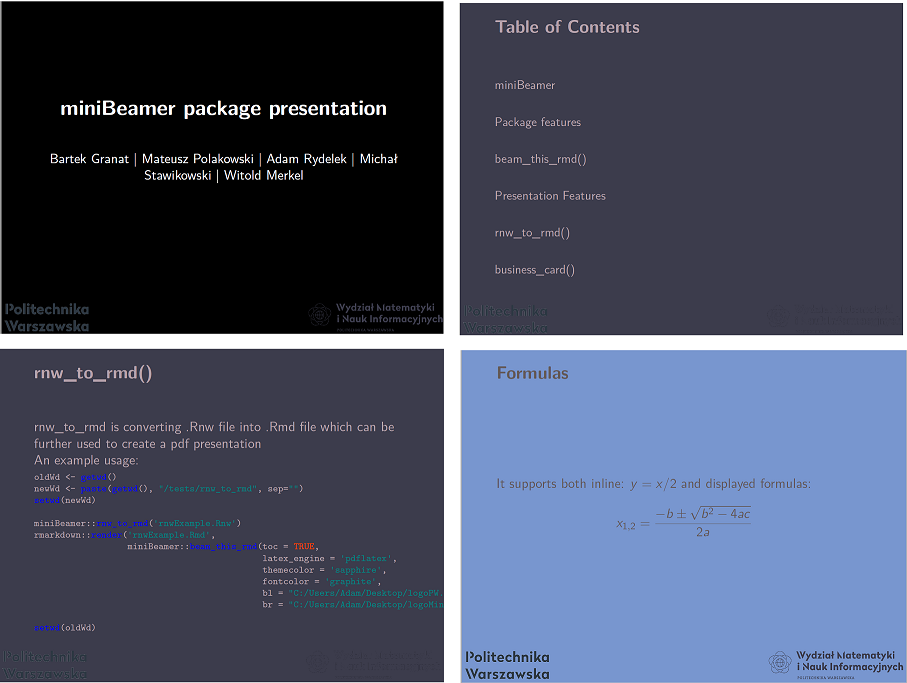
\includegraphics[width=3.43750in]{themes2.png}
\caption{Different themes}
\end{figure}

\end{frame}

\begin{frame}{Lists}

\begin{enumerate}
\def\labelenumi{\arabic{enumi}.}
\tightlist
\item
  11.11.2019 Stoachastic Processes exam
\item
  12.11.2019 HTML homework
\item
  1.01.2020 PARTY!!!
\end{enumerate}

\begin{itemize}
\tightlist
\item
  Drink juice
\item
  Eat popcorn
\item
  Go to sleep before midnight
\end{itemize}

\begin{enumerate}
\def\labelenumi{\arabic{enumi}.}
\tightlist
\item
  30.01.2020 ooops exams
\end{enumerate}

\end{frame}

\begin{frame}{Formulas}

It supports both inline: \(y = x / 2\) and displayed formulas:

\[ x_{1,2} = \frac{- b \pm \sqrt{b^2 - 4ac}}{2a} \]

\end{frame}

\begin{frame}{Slide with quote}

\begin{quote}
Na tym przedmiocie nie nauczę was jak się robi aplikację\ldots{} ale i
tak będziecie musieli ją zrobić.
\end{quote}

\textbf{Michał Okulewicz}

\end{frame}

\begin{frame}[fragile]{Slide with R Code and Output}

\scriptsize

\begin{Shaded}
\begin{Highlighting}[]
\KeywordTok{print}\NormalTok{(}\StringTok{'Test1'}\NormalTok{)}
\NormalTok{## [1] "Test1"}
\KeywordTok{options}\NormalTok{(}\DataTypeTok{tibble.width =} \DecValTok{120}\NormalTok{)}
\end{Highlighting}
\end{Shaded}

\begin{itemize}
\tightlist
\item
  Some text
\end{itemize}

\scriptsize

\begin{Shaded}
\begin{Highlighting}[]
\NormalTok{super_complicated_equation_evaluation <-}\StringTok{ }\DecValTok{2} \OperatorTok{+}\StringTok{ }\DecValTok{2}
\NormalTok{super_complicated_equation_evaluation}
\NormalTok{## [1] 4}
\end{Highlighting}
\end{Shaded}

\end{frame}

\begin{frame}{Tables}

\begin{longtable}[]{@{}cccc@{}}
\toprule
Przedmiot & Liczba godzin & ECTS &\tabularnewline
\midrule
\endhead
Analiza matematyczna 1 & 60 & 6 &\tabularnewline
HTML & 30 & 4 &\tabularnewline
Procesy Stochastyczne & 45 & 5 &\tabularnewline
Rachunek Prawdopodobieństwa & 60 & 6 &\tabularnewline
Zaawansowany R & 60 & 4 &\tabularnewline
\bottomrule
\end{longtable}

\end{frame}

\begin{frame}{Lists item by item}

\begin{enumerate}[<+->]
\def\labelenumi{\arabic{enumi}.}
\tightlist
\item
  Lets you reveal list items one by one
\item
  To keep some key points
\item
  In secret from audience
\item
  But it will work only once
\item
  Nobody wants to see the same joke twice
\end{enumerate}

\end{frame}

\begin{frame}{Never Gonna Give You Up}

\begin{figure}
\centering

\includegraphics{foto.jpg}
\caption{Super handsome Rick Astley}
\end{figure}

\end{frame}

\begin{frame}{Slide with Plot}

\scriptsize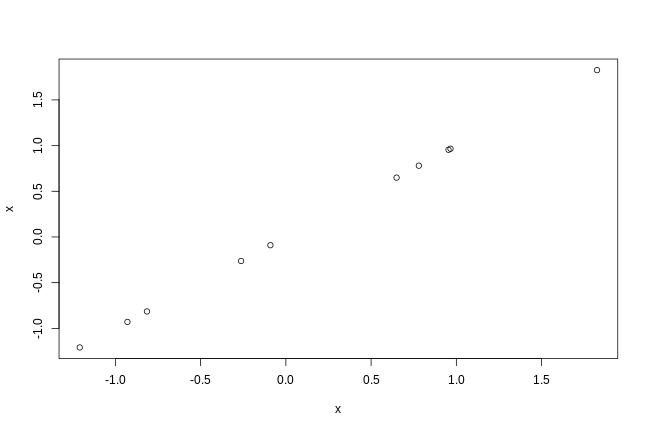
\includegraphics{prezentacja_pakietu_files/figure-beamer/unnamed-chunk-5-1.jpeg}

\end{frame}

\section{rnw\_to\_rmd()}\label{rnw_to_rmd}

\begin{frame}[fragile]{rnw\_to\_rmd()}

rnw\_to\_rmd is converting .Rnw file into .Rmd file which can be further
used to create a pdf presentation

An example usage:

\scriptsize

\begin{Shaded}
\begin{Highlighting}[]
\NormalTok{oldWd <-}\StringTok{ }\KeywordTok{getwd}\NormalTok{()}
\NormalTok{newWd <-}\StringTok{ }\KeywordTok{paste}\NormalTok{(}\KeywordTok{getwd}\NormalTok{(), }\StringTok{"/tests/rnw_to_rmd"}\NormalTok{, }\DataTypeTok{sep=}\StringTok{""}\NormalTok{)}
\KeywordTok{setwd}\NormalTok{(newWd)}

\NormalTok{miniBeamer}\OperatorTok{::}\KeywordTok{rnw_to_rmd}\NormalTok{(}\StringTok{'rnwExample.Rnw'}\NormalTok{)}
\NormalTok{rmarkdown}\OperatorTok{::}\KeywordTok{render}\NormalTok{(}\StringTok{'rnwExample.Rmd'}\NormalTok{, }
\NormalTok{                  miniBeamer}\OperatorTok{::}\KeywordTok{beam_this_rmd}\NormalTok{(}\DataTypeTok{toc =} \OtherTok{TRUE}\NormalTok{,}
                                            \DataTypeTok{latex_engine =} \StringTok{'pdflatex'}\NormalTok{,}
                                            \DataTypeTok{themecolor =} \StringTok{'sapphire'}\NormalTok{,}
                                            \DataTypeTok{fontcolor =} \StringTok{'graphite'}\NormalTok{,}
                                            \DataTypeTok{bl =} \StringTok{"C:/Users/Adam/Desktop/logoPW.jpg"}\NormalTok{,}
                                            \DataTypeTok{br =} \StringTok{"C:/Users/Adam/Desktop/logoMini.png"}\NormalTok{))}

\KeywordTok{setwd}\NormalTok{(oldWd)}
\end{Highlighting}
\end{Shaded}

\end{frame}

\section{business\_card()}\label{business_card}

\begin{frame}[fragile]{business\_Card()}

business\_card() is converting .Rmd file into beautiful MiNI WUT themed
business card

An example usage:

\scriptsize

\begin{Shaded}
\begin{Highlighting}[]
\NormalTok{rmarkdown}\OperatorTok{::}\KeywordTok{render}\NormalTok{(}
  \StringTok{'tests/business_card/business_card.Rmd'}\NormalTok{, miniBeamer}\OperatorTok{::}\KeywordTok{business_card}\NormalTok{()}
\NormalTok{)}
\end{Highlighting}
\end{Shaded}

\end{frame}

\begin{frame}[fragile]{Example business card}

\scriptsize

\begin{Shaded}
\begin{Highlighting}[]
\OperatorTok{---}
\NormalTok{address}\OperatorTok{:}\StringTok{ }\ErrorTok{|}
\StringTok{  }\ErrorTok{@}\NormalTok{mckraqs}
\NormalTok{logo}\OperatorTok{:}\StringTok{ "WMiNI-znak.png"}
\NormalTok{person}\OperatorTok{:}
\StringTok{  }\OperatorTok{-}\StringTok{ }\NormalTok{name}\OperatorTok{:}\StringTok{ }\NormalTok{Mateusz Polakowski}
\NormalTok{    title}\OperatorTok{:}\StringTok{ }\NormalTok{Data Science, MiNI PW}
\NormalTok{    phone}\OperatorTok{:}\StringTok{ "+48 997 998 999"}
\NormalTok{    email}\OperatorTok{:}\StringTok{ }\NormalTok{mateusz.polakowski}\OperatorTok{@}\NormalTok{mini.pw.edu.pl}
\NormalTok{    url}\OperatorTok{:}\StringTok{ }\NormalTok{https}\OperatorTok{:}\ErrorTok{//}\NormalTok{github.com}\OperatorTok{/}\NormalTok{mckraqs}\OperatorTok{/}\NormalTok{miniBeamer}
\NormalTok{cols}\OperatorTok{:}\StringTok{ }\DecValTok{1}
\NormalTok{rows}\OperatorTok{:}\StringTok{ }\DecValTok{1}
\NormalTok{output}\OperatorTok{:}\StringTok{ }\NormalTok{miniBeamer}\OperatorTok{::}\NormalTok{business_card}
\OperatorTok{---}
\end{Highlighting}
\end{Shaded}

\end{frame}

\begin{frame}{WOW! WOW! This card is nice!}

\begin{figure}
\centering

\includegraphics{card.png}
\caption{Business card}
\end{figure}

\end{frame}

\begin{frame}{Surprise}

\begin{figure}
\centering

\includegraphics{logo_beamer.png}
\caption{Hex}
\end{figure}

\end{frame}

% ***
% afterbody.tex template, feel free to use it
% File generated thanks to mckraqs/miniBeamer package!
% ***

\end{document}
